\documentclass[%
 reprint,
superscriptaddress,
%groupedaddress,
%unsortedaddress,
%runinaddress,
%frontmatterverbose, 
%preprint,
%preprintnumbers,
 nofootinbib,
%nobibnotes,
%bibnotes,
 amsmath,amssymb,
 aps,
 prd,
%prb,
%rmp,
%prstab,
%prstper,
%floatfix,
]{revtex4-2}

%---------- Packages ----------
\usepackage{xcolor}
\usepackage{multirow}
% \usepackage{tabularx}
\usepackage{graphicx}% Include figure files
\usepackage{dcolumn}% Align table columns on decimal point
\usepackage{bm}% bold math
\usepackage{acronym}
\usepackage{hyperref}
\usepackage{orcidlink}
\usepackage{array}

%---------- Colours ----------
\definecolor{garibaldired}{HTML}{DD0000}
\newcommand{\gscd}[1]{\textcolor{garibaldired}{[\textbf{GCD}: #1]}}
\newcommand{\iwh}[1]{\textcolor{magenta}{[\textbf{IWH}: #1]}}

\newcommand{\strutrow}{\rule{0pt}{2.5ex}} % This gives a little extra space in tables
\newcommand{\portsmouth}{Institute of Cosmology \& Gravitation, University of Portsmouth, Portsmouth, United Kingdom}

%---------- Document ----------
\begin{document}

\preprint{APS/123-QED}

\title{Inpainting over the cracks: challenges of applying pre-merger searches for massive black hole binaries to realistic LISA datasets}

\author{Gareth {Cabourn Davies}\orcidlink{0000-0002-4289-3439}}
\email{gareth.cabourn-davies@port.ac.uk}
\affiliation{\portsmouth}
\author{Ian Harry\orcidlink{0000-0002-5304-9372}}
\email{ian.harry@port.ac.uk}
\affiliation{\portsmouth}

\begin{abstract}
    A key science target of the Large Interferometer Space Antenna (LISA) is to carry out
    multi-messenger observations of massive black hole binaries, observing the merger
    simulataneously in gravitational waves and with electromagnetic observatories.
    Identifying that a merger is happening and providing an updating estimate of the sky location in the hours, days and weeks before the merger is critical to enable electromagnetic observations of the merger event. 
    In this work we demonstrate and compare two methods for premerger identification of massive
    black hole binaries; a zero-latency filter approach and, for the first time, an approach using an ``inpainting'' technique.
    We apply these methods to the LISA Data Challenge dataset 2a: Sangria-HM and demonstrate the
    successful recovery of the 14 signals in the dataset that we expected to be identifiable at
    least half a day before merger.
    We demonstrate that the inpainting method can identify premerger signals even when gaps are present in the data, demonstrating the recovery of signal 0 even when 3 day-long data gaps are added to the 14 days preceding merger.
    Finally, we explore the challenge of overlapping signals, using signals 2 - 5, all of which merge within a 10-day window, and show how removing signals that have been confidently identified from the data allows us to identify quieter signals in the same period.
\end{abstract}

\maketitle

% Credit statement as a footnote beneath the emails
\begingroup
    \renewcommand\thefootnote{}
    \footnotetext{Both authors contributed equally to this work.}
    \addtocounter{footnote}{-1}
\endgroup

\acrodef{LISA}[LISA]{Laser Interferometer Space Antenna}
\acrodef{MBHB}[MBHB]{Massive Black Hole Binary}
\acrodefplural{MBHB}[MBHBs]{Massive Black Hole Binaries}
\acrodef{WD}[WD]{White Dwarf}
\acrodef{GB}[GB]{Galactic Binary}
\acrodefplural{GB}[GBs]{Galactic Binaries}
\acrodef{PSD}[PSD]{Power Spectral Density}
\acrodefplural{PSD}[PSDs]{Power Spectral Densities}
\acrodef{ASD}[ASD]{Amplitude Spectral Density}
\acrodefplural{ASD}[ASDs]{Amplitude Spectral Densities}
\acrodef{FAR}{false alarm rate}
\acrodef{SNR}{signal-to-noise ratio}

\section{Introduction}
\label{sec:intro}

The \ac{LISA} gravitational-wave observatory, planned for launch in the mid-to-late
2030s~\cite{LISA:2017pwj, Colpi:2024xhw}, will unlock our ability to observe the universe
in the low-frequency gravitational-wave band~\cite{LISA:2022yao}.

A key science target
for \ac{LISA} is the observation of \acp{MBHB}. The problem of observing and characterizing
these mergers has been explored over the last two decades, primarily through the LISA Data
Challenges~\cite{Arnaud:2006gm, MockLISADataChallengeTaskForce:2006sgi, Arnaud:2007vr,
MockLISADataChallengeTaskForce:2007iof, Babak:2008aa, Arnaud:2007jy,
MockLISADataChallengeTaskForce:2009wir, Baghi:2022ucj, LDC_WEBSITE}. Because these signals will
have a very large \ac{SNR}, the search for these sources is
expected to be trivial~\cite{LISA:2022yao}.
 
A particularly powerful capability of \ac{LISA} is the detection of these \ac{MBHB} systems
in the weeks to months before they merge~\cite{CabournDavies:2024hea, Houba:2024mqj,
Ruan:2024qch}. Such \textit{pre-merger} observations can provide early warnings and sky-localisation
estimates~\cite{CabournDavies:2024hea, Kocsis:2007yu, McWilliams:2011zs, Saini:2022hrs}
for these incredibly science-rich events~\cite{DalCanton:2019wsr}.
This advanced notice is critical to enable multi-messenger astronomy, allowing
electromagnetic facilities to be directed toward the source region rapidly to maximise observation.

In contrast to prevailing methods for pre-merger \ac{MBHB} observation, which often rely on
Fisher Matrix analyses or Bayesian inference with abruptly terminated waveforms, our
technique introduced in~\cite{CabournDavies:2024hea} offers a more immediate analysis. It allows
for the accurate computation of a matched filter without the need to wait (up to a day) for
additional data to arrive. After this data has arrived, the observation window may have passed, or
\ac{LISA} itself may have been turned off for repositioning or data downlink.

In this paper, we present application of this technique to the latest data challenge dataset,
Sangria-HM in Section~\ref{sec:zerolatency_sangria}, showing the potential pitfalls of na\"ive implementation
of the search.

These pitfalls lead us to consider utilising the inpainting technique of~\cite{Zackay:2019kkv} as an
alternative to the zero-latency filter of~\cite{CabournDavies:2024hea}. This is described in
Section~\ref{sec:inpainting}, and applied it in Section~\ref{sec:inpainting_sangria}.

All of our results and figures are fully reproducible, with the code
used to make them publicly available. Please see the data release at
\url{https://icg-gravwaves.github.io/lisa_premerger_sangria/}
for more detail.


\subsection{Noise Estimation}
\label{subsec:psds}
Our first consideration is to check whether the data from the Sangria dataset has
similar noise properties to the datasets used our previous work. 
\gscd{How does the Sangria dataset compare to the PSDs that we used to set up the zerolatency filter banks?}

\begin{figure*}
    \centering
    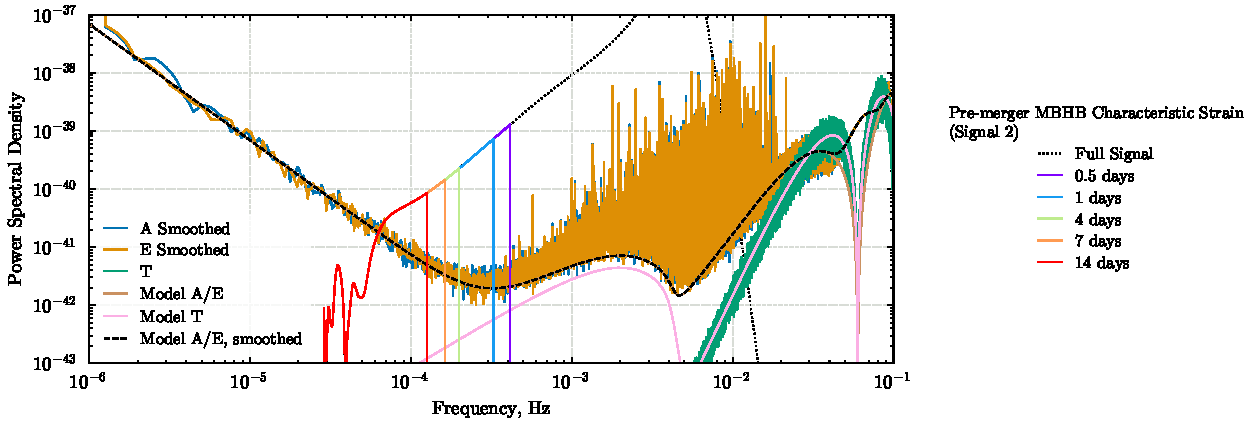
\includegraphics[width=\textwidth]{images/figure_X_psds_with_sources.pdf}
    \caption{
        Comparison of PSDs used in this work.
        The PSD is estimated from the Sangria dataset using the welch method with a segment duration of 18.25 days.
        The model shown is the noise model used to produce the Sangria dataset, and includes unresolvable galactic binary sources.
        Both the model and the estimated PSD require smoothing over the dip to zero at 0.06Hz.
        This smoothing is done using a Hann window to transition between the original PSD and a straight line between the peaks of the PSD model either side of the dip.
        We also show the characteristic strain for a MBHB signal from Sangria (Signal 4), which shows that at 14, 7 and 4 days-before-merger, the MBHB does not overlap
        the galactic binary confusion noise in frequency, but when the signal reaches around one day before merger,
        the galactic binary confusion noise starts to overlap with the signal.
    }
    \label{fig:psds}
\end{figure*}

\begin{table*}
    \begin{tabular}{|cc|c|ccccc|}
\hline
\multicolumn{2}{|c|}{Signal}& \multicolumn{6}{c|}{Expected SNR} \\
\hline
Number & Time  & Full Signal & 0.5 & 1 & 4 & 7 & 14 \\
\hline
0 & 55.56 & 2699.04 & 70.99 & 52.74 & 24.33 & 16.43 & 9.51 \\
1 & 101.23 & 105.72 & 3.99 & 2.49 & 0.79 & 0.47 & 0.28 \\
2 & 129.26 & 400.25 & 10.76 & 7.51 & 2.91 & 1.84 & 1.07 \\
3 & 130.31 & 1992.38 & 71.92 & 54.76 & 27.52 & 19.88 & 13.22 \\
4 & 133.41 & 3475.28 & 115.99 & 88.26 & 44.02 & 31.65 & 20.46 \\
5 & 138.55 & 427.13 & 16.40 & 10.79 & 3.85 & 2.37 & 1.22 \\
6 & 157.61 & 673.48 & 24.99 & 16.19 & 5.48 & 3.25 & 1.55 \\
7 & 191.34 & 579.12 & 15.72 & 10.70 & 4.02 & 2.56 & 1.49 \\
8 & 199.60 & 365.18 & 16.21 & 10.68 & 3.77 & 2.28 & 1.11 \\
9 & 215.34 & 392.96 & 18.69 & 12.41 & 4.75 & 3.12 & 1.82 \\
10 & 236.41 & 2187.78 & 45.09 & 31.90 & 12.71 & 8.13 & 4.37 \\
11 & 257.27 & 1200.55 & 45.32 & 33.31 & 13.99 & 8.92 & 4.71 \\
12 & 271.29 & 359.02 & 21.27 & 14.71 & 6.10 & 4.17 & 2.57 \\
13 & 282.51 & 823.00 & 24.75 & 18.00 & 7.81 & 5.23 & 3.00 \\
14 & 341.62 & 230.57 & 9.88 & 6.43 & 2.22 & 1.34 & 0.67 \\
\hline
\end{tabular}

    \caption{
        Characteristic SNRs for signals in the Sangria dataset.
        These are computed by comparing characteristic strain for the signal to the
        noise model PSD.
        We see that Signals 5 and 14 are unlikely to be seen even 0.5 days pre-merger, and 
        that signals 
    }
    \label{tab:characteristic_strain_snr}
\end{table*}

As a result, we can use the template banks from the zero-latency search paper without significant issues.



\section{The Sangria HM Dataset}
\label{sec:dataset}

We test our search methods on the LISA Data Challenge dataset~\cite{Baghi:2022ucj, LDC_WEBSITE}.
The LISA Data Challenges are designed to provide comprehensively modelled data as an introduction
to LISA data analysis. The dataset considered here is Challenge 2a, also known as
\textit{Sangria-HM}~\cite{LDC_WEBSITE_SANGRIA_HM}.
This dataset is similar to Challenge 2: Sangria~\cite{LDC_WEBSITE_SANGRIA, le_jeune_2022_7132178};
it contains exactly the same sources but uses a different waveform model, \texttt{PhenomHM}~\cite{}
... \gscd{A couple more sentences of introduction to sangria}

In applying our pre-merger search to the Sangria dataset, our first consideration is to check whether
the data has similar noise properties to our assumptions in our previous work. 
Figure~\ref{fig:psds} shows the PSD  

\begin{figure*}
    \centering
    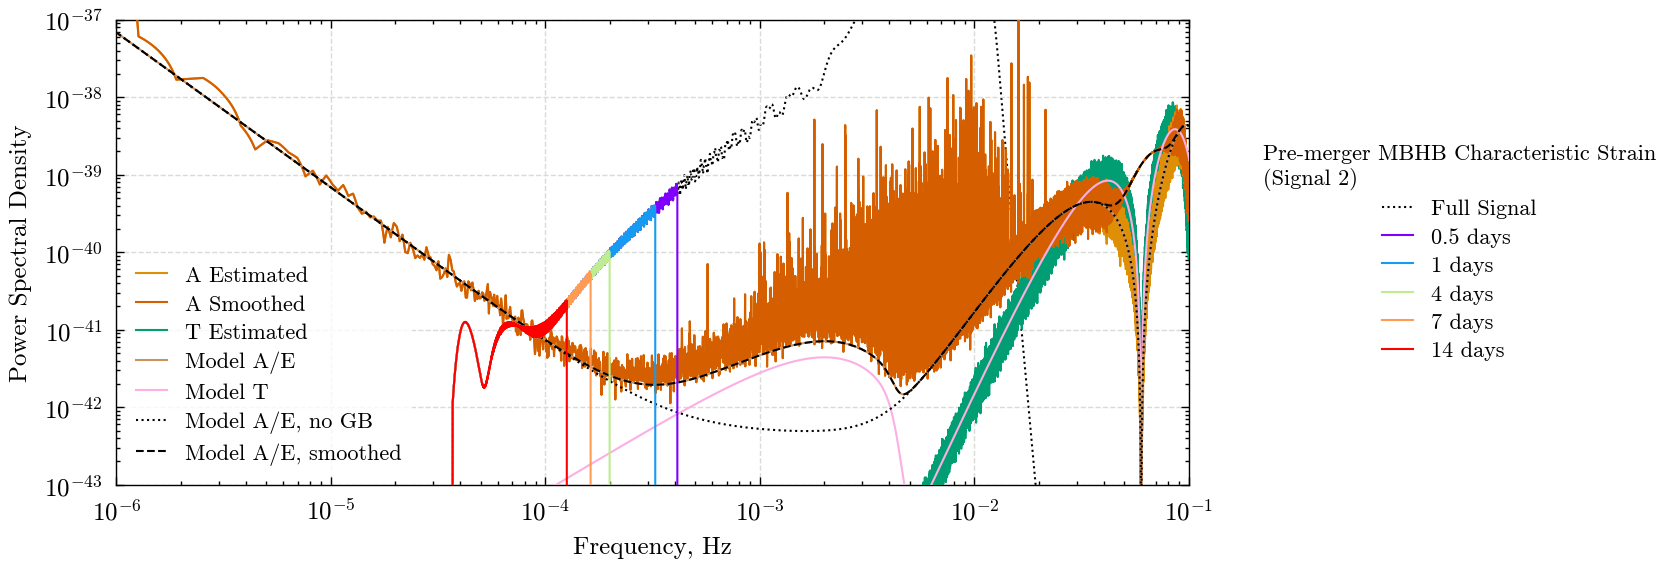
\includegraphics[width=\textwidth]{images/dataset/figure_X_psds_with_sources.png}
    \caption{
        Comparison of PSDs used in this work.
        The PSD is estimated from the Sangria dataset using the welch method with a segment duration of 18.25 days.
        The model shown is the noise model used to produce the Sangria dataset, and includes unresolvable galactic binary sources.
        Both the model and the estimated PSD require smoothing over the dip to zero at 0.06Hz.
        This smoothing is done using a Hann window to transition between the original PSD and a straight line between the peaks of the PSD model either side of the dip.
        We also show the characteristic strain for a representative MBHB signal from Sangria (Signal 2), which shows that at 14, 7 and 4 days-before-merger, the MBHB does not overlap
        the galactic binary confusion noise in frequency, but when the signal reaches around one day before merger,
        the galactic binary confusion noise starts to overlap with the signal.
    }
    \label{fig:psds}
\end{figure*}

\begin{table}
    \begin{tabular}{|cc|c|ccccc|}
\hline
\multicolumn{2}{|c|}{Signal}& \multicolumn{6}{c|}{Expected SNR} \\
\hline
Number & Time  & Full Signal & 0.5 & 1 & 4 & 7 & 14 \\
\hline
0 & 55.56 & 2699.04 & 70.99 & 52.74 & 24.33 & 16.43 & 9.51 \\
1 & 101.23 & 105.72 & 3.99 & 2.49 & 0.79 & 0.47 & 0.28 \\
2 & 129.26 & 400.25 & 10.76 & 7.51 & 2.91 & 1.84 & 1.07 \\
3 & 130.31 & 1992.38 & 71.92 & 54.76 & 27.52 & 19.88 & 13.22 \\
4 & 133.41 & 3475.28 & 115.99 & 88.26 & 44.02 & 31.65 & 20.46 \\
5 & 138.55 & 427.13 & 16.40 & 10.79 & 3.85 & 2.37 & 1.22 \\
6 & 157.61 & 673.48 & 24.99 & 16.19 & 5.48 & 3.25 & 1.55 \\
7 & 191.34 & 579.12 & 15.72 & 10.70 & 4.02 & 2.56 & 1.49 \\
8 & 199.60 & 365.18 & 16.21 & 10.68 & 3.77 & 2.28 & 1.11 \\
9 & 215.34 & 392.96 & 18.69 & 12.41 & 4.75 & 3.12 & 1.82 \\
10 & 236.41 & 2187.78 & 45.09 & 31.90 & 12.71 & 8.13 & 4.37 \\
11 & 257.27 & 1200.55 & 45.32 & 33.31 & 13.99 & 8.92 & 4.71 \\
12 & 271.29 & 359.02 & 21.27 & 14.71 & 6.10 & 4.17 & 2.57 \\
13 & 282.51 & 823.00 & 24.75 & 18.00 & 7.81 & 5.23 & 3.00 \\
14 & 341.62 & 230.57 & 9.88 & 6.43 & 2.22 & 1.34 & 0.67 \\
\hline
\end{tabular}

    \caption{
        Characteristic SNRs for signals in the Sangria dataset.
        These are computed by comparing characteristic strain for the signal to the
        noise model PSD.
        We see that Signal 1 is unlikely to be seen even 0.5 days pre-merger, and 
        that only the loudest signals - 0, 3, 4, 10, 11 and possibly 12, 13 - would be seen 4 days before merger.
    }
    \label{tab:characteristic_strain_snr}
\end{table}

\subsection{Smoothing the PSD}
PSD goes to zero at 60mHz - problem!

\begin{figure}
    \centering
    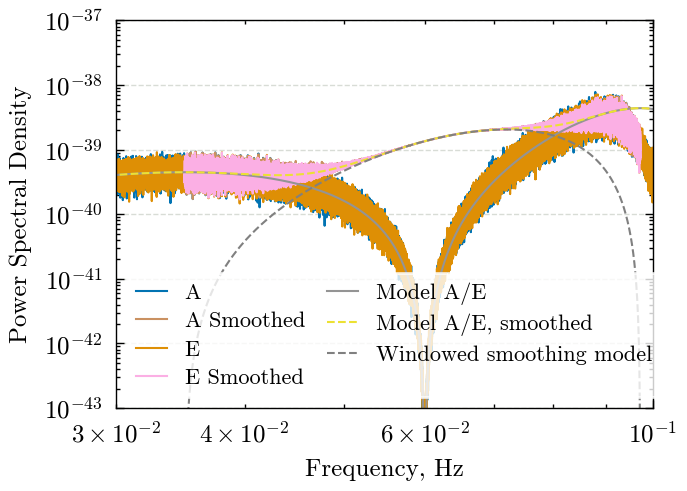
\includegraphics[width=\columnwidth]{images/dataset/figure_X_smoothing_60mHz.png}
    \caption{
        The method used to smooth over the dip in the PSD at 60 mHz.
        We draw a straight line between the two peaks either side of this point, and smoothly
        This ensures that there are no immediate jumps in the PSD to cause spectral leakage.
        transition betweem the estimated PSD and the straight line using a Hann window.
        This is applied to both the estimated and modelled PSDs used in later analysis.
    }
    \label{fig:smoothing}
\end{figure}



\section{Applying the Premerger Search}
\label{sec:zerolatency_sangria}

Our search uses a zero-latency filter such that data from the future is not required. A full
description is in~\cite{CabournDavies:2024hea}, and is based on work from~\cite{Tsukada:2017cuf}.

We apply this search to the LISA Data Challenge dataset~\cite{Baghi:2022ucj, LDC_WEBSITE}.
The LISA Data Challenges are designed to provide comprehensively modelled data as an introduction
to LISA data analysis. The dataset considered here is Challenge 2a, also known as
\textit{Sangria-HM}~\cite{LDC_WEBSITE_SANGRIA_HM}.
This dataset is similar to Challenge 2: Sangria~\cite{LDC_WEBSITE_SANGRIA, le_jeune_2022_7132178};
it contains exactly the same sources but uses a different waveform model, \texttt{PhenomHM}~\cite{}
... \gscd{A couple of sentences of introduction to sangria - maybe this isnt a subsection?}

To apply this search, we set up the data so that we can truncate it, this was done in hourly intervals,
and then apply the search at 14, 7, 4 and 1 days before merger.

\subsection{Noise Estimation}
\label{subsec:psds}
Our first consideration is to check whether the data from the Sangria dataset has
similar noise properties to the datasets used our previous work. 
\gscd{How does the Sangria dataset compare to the PSDs that we used to set up the zerolatency filter banks?}

\begin{figure*}
    \centering
    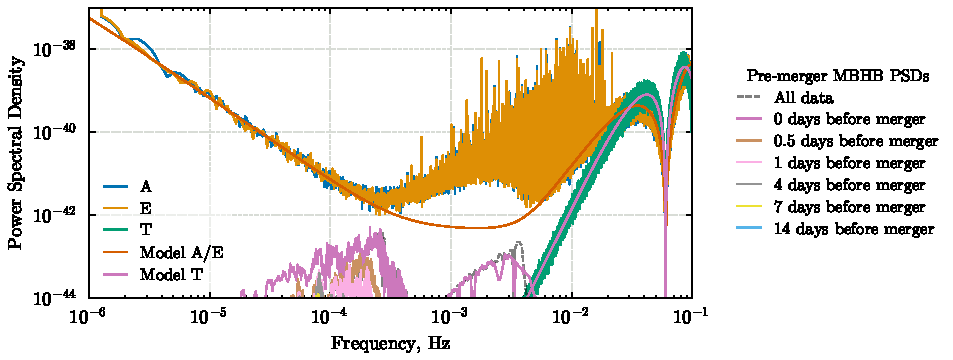
\includegraphics[0.75\textwidth]{images/figure_X_psds_with_premerger_mbhbs.pdf}
    \caption{}
    \label{fig:psds}
\end{figure*}

As a result, we can use the template banks from the zero-latency search paper without significant issues.

\subsection{Secondary Peaks in Signal-to-Noise Ratio}
\label{subsec:double_peaks}
\gscd{Discussion of finding the secondary peaks in the SNR.}

\subsection{Secondary Peak Removal}
\label{subsec:peak_removal}
\gscd{Removing the peaks, and the results of the search including removing the peaks. Discussion of whether assuming that the signal is known is valid or not}

Signal 1 appears to now be missed in the plot, however the former peak in SNR is from the 0.5 days after merger analysis
matching to the peak itself.
Signal 5 can now be seen, as the contamination from the louder Signal 4 is now no longer a problem.

\subsection{Search Results}
\label{subsec:zerolatency_results}
\gscd{Discussion of the analysis results}

\section{Inpainting}
\label{sec:inpainting}

\iwh{This section should contain the theoretical motivation behind inpainting and the details of how it is applied \emph{in general}. I'm trying to work on this at the moment.}

\gscd{Need to be somewhat careful here, as it doesnt particularly follow on from the zerolatency filter method.
Motivate its use first, then go into details}

We have showed in the previous section, and in our previous work~\cite{CabournDavies:2024hea}, that the zero-latency filter method, used successfully for many years in ground-based low-latency analysis~\cite{Tsukada:2017cuf} is directly applicable to
solve the \ac{MBHB} premerger problem in LISA.

However, when considering the case of LISA, there are some issues with this method that warrant considering alternatives. The premerger analysis that we carried out with the zero-latency filter here analyzes 30 days of data to identify mergers up to 14 days before merger. LISA data is expected to have gaps \iwh{say a bit about expected cadence of gaps and cite some LISA design/white paper}. We do not have a method for dealing with these gaps using the zero-latency filter and therefore if there is a gap in the recorded LISA data in the days before a \ac{MBHB} merger it might result in a delay in identifying that the merger is about to happen.

Here we consider an alternative technique, which is also adapted from ground-based analyses. In particular the observation of the first binary neutron star merger, GW170817, was significantly hampered by the presence of a loud non-Gaussian artefact in the seconds before the merger. At the time of observation the glitch was manually excised from the data, in a process known as "gating". However, this gating might result in spectral leakage in the whitened strain, as described in~\cite{Zackay:2019kkv}, which can cause issues for detection pipelines and bias inference algorithms.

The method of ``inpainting'' for proposed in~\cite{Zackay:2019kkv} as an
alternative for safely removing non-Gaussianities or, equivalently, for analysing over data gaps. The full derivation is given in~\cite{Zackay:2019kkv,Capano:2021etf} but the basic idea is that we want the ``overwhitened'' strain to be 0s for the duration of the gap. If we consider the matched-filter between signal, $s$ and data $h$
%
\begin{equation}
    (h|s) = 4\mathrm{Re}\int_{f_\mathrm{low}}^{f_\mathrm{high}}\frac{\tilde{h}(f)\tilde{s}^*(f)}{S_n(f)} \mathrm{d} f,
\end{equation}
%
we can rewrite this as
%
\begin{equation}
    (h|s) = 4\mathrm{Re}\int_{f_\mathrm{low}}^{f_\mathrm{high}} \tilde{h}(f) \frac{\tilde{s}^*(f)}{S_n(f)} \mathrm{d} f,
\end{equation}
%
where $\tilde{s}^*(f) / S_n(f)$ is the ``overwhitened'' strain. The matched-filter is then the cross correlation between the overwhitened strain and the template waveform and therefore any 0s in the overwhitened strain will not contribute to the overall matched-filter. Choosing values that the data should take in the gap of the [unwhitened] strain such that the overwhitened strain is 0 boils down to a linear algebra problem.


Gaps in the data will cause significant issue in the \ac{LISA} data analysis\gscd{CITE}, and there is not a way to
implement the zero-latency filter method to account for multiple gaps in the data.
As a result, we consider the use of \textit{inpainting} - a data analysis technique used to fill in missing
segments of detector data~\cite{Zackay:2019kkv}.
\gscd{This is probably where we can really big up inpainting - the zerolatency filter method can't deal with data gaps.}

To describe inpainting, we consider matched filtering, and how the removal of data in each term
must be considered.

The basic \ac{SNR} calculation is
\begin{equation}
    \rho^2(t) = \frac{[(h|s)]^2}{(h|h)}
\end{equation}

where the inner product is
\begin{equation}
    (a|b)(t) = 4\mathrm{Re}\int_{f_\mathrm{low}}^{f_\mathrm{high}}\frac{\tilde{a}(f)\tilde{b}^*(f)}{S_n(f)} \mathrm{e}^{2i \pi ft} \mathrm{d} f,
\end{equation}

$\tilde{a}$ defines the Fourier transform, $\tilde{b}^*(f)$ is the complex conjugate 
of the Fourier transform, and $S_n(f)$ is the one-sided \ac{PSD} of the detector noise.

\subsection{$(h|s)$}
\label{subsubsec:h_s}
Dividing the data $\tilde{s}(f)$ by the square root of the \ac{PSD} - the \ac{ASD}, $\sqrt{S_n(f)}$ -
of the noise is often referred to as \textit{whitening} the data, as the spectral density of the data will
become flat by this procedure. By performing this step twice on the data, we produce \textit{overwhitened} data
\footnote{Also sometimes refered to as \textit{blued} data, particularly in \cite{Zackay:2019kkv}}.
With overwhitened data, we are able to use un-whitened templates in the inner product calculation.

The method of inpainting is to add values to the gap so that after the overwhitening procedure, data outside
the gap time is unaffected, but data within the gap becomes zero. If the data within the gap can be identically
zero after overwhitening, then the data from this time will not contribute to the \ac{SNR} calculation.

The challenge to calculate the values to be added to the gap is one of linear algebra, fully described
in~\cite{Zackay:2019kkv}, and implementated in \texttt{PyCBC} for~\cite{Capano:2021etf,Wang:2023ljx}, 

\subsection{$(h|h)$}
\label{subsubsec:h_h}


\subsection{Use as a Premerger Search}
\label{subsec:inpainting_premerger}
Inpainting does not require data either side in order to `bridge' a gap, and so
we can consider the missing data in the future to simply be a one-sided gap.

For ringdown analyses, once can use inpainting to remove data from the inspiral~\cite{Capano:2021etf,Wang:2023ljx},
so that the masses and spins can be inferred independently from the ringdown and inspiral, and cross-checked.
Here, we propose a similar strategy, but removing data from the opposite end; by inpainting and setting all
future data to zero, we can - similarly to~\cite{CabournDavies:2024hea} - implement a pre-merger search without
the requirement to wait for future data.
This solution works for LISA but not ground-based premerger searches \gscd{CITE!} as the speed requirements of
ground-based pre-merger analyses mean that we cannot wait for teh inpainting procedure in real time \gscd{word this better}

\section{Paint Application}
\label{sec:inpainting_sangria}

\iwh{This should mostly discuss the inpainting results. A brief discussion
of the template bank we used is needed perhaps alongside how one might improve this in the future. However, the focus here is results. We want to show that we still observe X signals, but now we want to have numbers that are not 14/7/4/1 but 13.56 or whatever. Some nice plots showing the overall picture will also be useful. As before, leave the dense region}

\iwh{THEN add a new section called "overlapping signals" or similar and present the focused region and how the various searches have handled this. The timetable within the inpainting search where it finds signal 3 \emph{before} signal 2 is important to show nicely here as well.}

\gscd{The application of inpainting to the Sangria Dataset. Maybe have a scatter plot of the hourly results showing inpainting vs the zerolatency Filter (with removal)}

\subsection{Template Banks}
\label{subsec:inpainting_banks}

\subsection{Search Results}
\label{subsec:inpainting_results}

\section{Overlapping Signals}
\label{sec:focused}

\begin{figure}
    \centering
    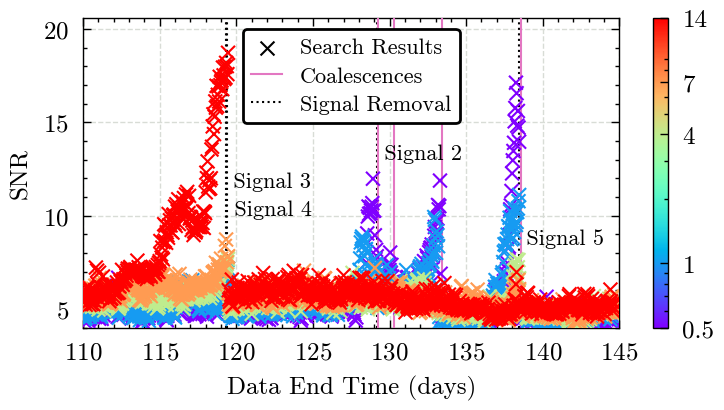
\includegraphics[width=\columnwidth]{images/inpainting_results/figure_X_focused_region_variable_removal.png}
    \caption{
        Timeline of results in the congested period of days 110-140 of the Sangria Dataset
    }
    \label{fig:variable_removal}
\end{figure}


\section{Conclusion and Discussion}
\label{sec:conclusion}

\gscd{Conclusions, possible future work, application to inference etc.}

\begin{acknowledgments}
For the purpose of open access, the authors have applied a Creative Commons Attribution (CC-BY)
licence to any author accepted manuscript version arising from this submission.

This work was supported by a series of UKSA grants
supporting the UK's contribution to LISA's Ground
Segment activities.
GCD and IH acknowledge support from \gscd{FIXME}

The authors are grateful for computational resources provided
by Cardiff University, and funded by STFC awards supporting
UK Involvement in the Operation of Advanced LIGO.
Numerical computations were also carried out on the Sciama High
Performance Computing (HPC) cluster, which is supported by the
Institute of Cosmology and Gravitation, the South-East Physics
Network (SEPNet) and the University of Portsmouth.

\textit{Software} This work made use of the following software packages:
\texttt{BBHx}~\cite{michael_katz_2023_7791640},
\texttt{GstLAL}~\cite{Cannon:2020qnf},
\texttt{matplotlib}~\cite{Hunter:2007},
\texttt{numpy}~\cite{harris2020array},
\texttt{PyCBC}~\cite{alex_nitz_2024_10473621},
\texttt{scipy}~\cite{2020SciPy-NMeth}

\gscd{Should we include this or not? I feel that we should include something like this}
Large Language Models were used in this work to generate code snippets efficiently,
debug errors, and provide editing assistance in the writing of this manuscript.

\end{acknowledgments}

\bibliography{bibliography}

\appendix

\section{Power loss due to Galactic Binary foreground}
\label{sec:gb_noise_snr_loss}
\updated{As demonstrated in Figure~\ref{fig:psds}, the pre-merger analysis mainly cuts off before the galactic bnary confusion noise becomes significant.}

\updated{Here we calculate how much SNR is lost due to the Galactic Binary confusion noise for each signal.}

\begin{figure}
   \centering
   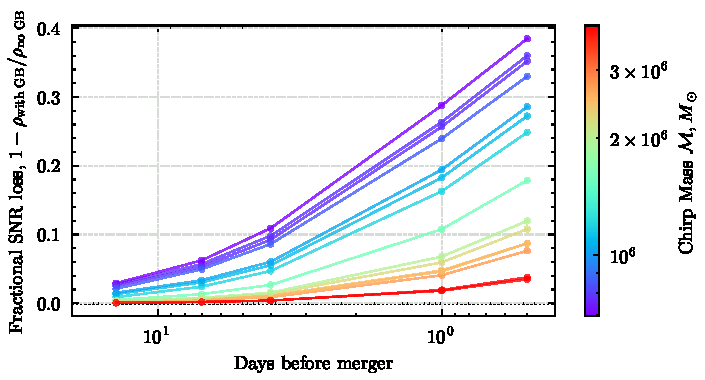
\includegraphics[width=\columnwidth]{images/figure_12_GB_SNR_loss.pdf}
   \caption{
       \updated{Fractional signal-to-noise ratio loss for each signal caused by Galactic Binary confusion noise.
       We see that signals at lower chirp masses are affected more, losing up to 39\% of power half a day before merger.
       For heavier signals, and for times more than a few days before merger, the signal power loss is much less, below 10\%.}
   }
   \label{fig:removal_residual}
\end{figure}

\section{Signal Removal}
\label{sec:signal_removal}
\updated{As discussed in Section~\ref{sec:focused}, the loudest signals from the data can match to templates in the bank even with the small amount of template power away from the merger.
The solution is to manually remove signals from the data as soon as they are known.
This is similar to the global fit challenge, but remains within the same source type.
To remove signals from the data, we assume that the signal is known perfectly, and the parameters of the injection are use to generate a waveform which is subtracted from the data.}

\updated{As shown in Figure~\ref{fig:removal_residual}, signal removal is not perfect, and some signal power remains.
We encourage the release of the exact methods which were used to produce the datasets so that they can be independently recreated.}

\begin{figure}
   \centering
   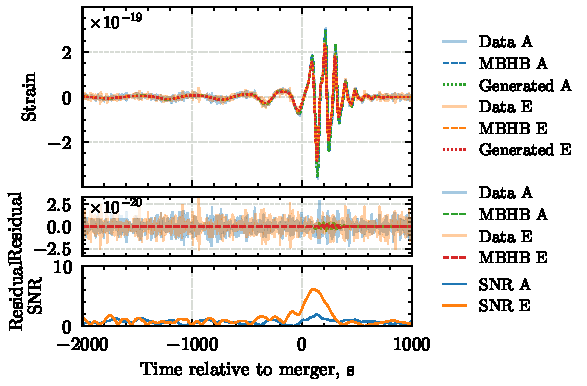
\includegraphics[width=\columnwidth]{images/figure_11_removal_residual.pdf}
   \caption{
       \updated{Residuals after removal for Signal 3.
       Equivalent plots for all signals are included in the data release.}
   }
   \label{fig:removal_residual}
\end{figure}

\updated{The remaining signal power still produces a small signal-to-noise ratio peak, as in Figure~\ref{fig:variable_removal}.
Early estimate parameter estimation routines may find parameters which remove more of the signal from the data, and so this may not be an issue in real LISA premerger analyses.}

\end{document}